%%%%%%%%%%%%%%%%%%%%%%%%%%%%%%%%%%%%%%%%%
% Beamer Presentation
% LaTeX Template
% Version 1.0 (10/11/12)
%
% This template has been downloaded from:
% http://www.LaTeXTemplates.com
%
% License:
% CC BY-NC-SA 3.0 (http://creativecommons.org/licenses/by-nc-sa/3.0/)
%
%%%%%%%%%%%%%%%%%%%%%%%%%%%%%%%%%%%%%%%%%

%----------------------------------------------------------------------------------------
%	PACKAGES AND THEMES
%----------------------------------------------------------------------------------------

\documentclass{beamer}

\mode<presentation> {

% The Beamer class comes with a number of default slide themes
% which change the colors and layouts of slides. Below this is a list
% of all the themes, uncomment each in turn to see what they look like.

%\usetheme{default}
%\usetheme{AnnArbor}
%\usetheme{Antibes}
%\usetheme{Bergen}
%\usetheme{Berkeley}
%\usetheme{Berlin}
%\usetheme{Boadilla}
%\usetheme{CambridgeUS}
%\usetheme{Copenhagen}
%\usetheme{Darmstadt}
%\usetheme{Dresden}
%\usetheme{Frankfurt}
%\usetheme{Goettingen}
%\usetheme{Hannover}
%\usetheme{Ilmenau}
%\usetheme{JuanLesPins}
%\usetheme{Luebeck}
%\usetheme{Madrid}
%\usetheme{Malmoe}
%\usetheme{Marburg}
\usetheme{Montpellier}
%\usetheme{PaloAlto}
%\usetheme{Pittsburgh}
%\usetheme{Rochester}
%\usetheme{Singapore}
%\usetheme{Szeged}
%\usetheme{Warsaw}

% As well as themes, the Beamer class has a number of color themes
% for any slide theme. Uncomment each of these in turn to see how it
% changes the colors of your current slide theme.

%\usecolortheme{albatross}
%\usecolortheme{beaver}
%\usecolortheme{beetle}
%\usecolortheme{crane}
%\usecolortheme{dolphin}
%\usecolortheme{dove}
%\usecolortheme{fly}
%\usecolortheme{lily}
%\usecolortheme{orchid}
%\usecolortheme{rose}
%\usecolortheme{seagull}
%\usecolortheme{seahorse}
%\usecolortheme{whale}
%\usecolortheme{wolverine}

%\setbeamertemplate{footline} % To remove the footer line in all slides uncomment this line
%\setbeamertemplate{footline}[page number] % To replace the footer line in all slides with a simple slide count uncomment this line

%\setbeamertemplate{navigation symbols}{} % To remove the navigation symbols from the bottom of all slides uncomment this line
}

\usepackage{graphicx} % Allows including images
\usepackage{booktabs} % Allows the use of \toprule, \midrule and \bottomrule in tables

%----------------------------------------------------------------------------------------
%	TITLE PAGE
%----------------------------------------------------------------------------------------

\title[Mastering Metrics]{Understanding Metrics based on Mastering Metrics } % The short title appears at the bottom of every slide, the full title is only on the title page

\author{Corinna Birner \& Max M{\"u}ller} % Your name
\institute[JMU] % Your institution as it will appear on the bottom of every slide, may be shorthand to save space
{University of W{\"u}rzburg }\\ % Your institution for the title page
\medskip
\textit{{corinna.birner@stud-mail.uni-wuerzburg.de 
max.mueller@stud-mail.uni-wuerzburg.de} % Your email address
}
\date{\today} % Date, can be changed to a custom date

%------------------------------------------------
\begin{document}

\begin{frame}
\titlepage % Print the title page as the first slide
\end{frame}

%------------------------------------------------
\begin{frame}
\begin{center}
\textbf\Huge{Chapter 1: Randomized Trials}
\end{center}
\end{frame}

%------------------------------------------------
\begin{frame}
\frametitle{Overview} % Table of contents slide, comment this block out to remove it
Today we will start our journey on the path from cause to effect. Therefore, we will discuss randomized trials as one possible way of finding causal relations in data. Our topics will be the following:

\tableofcontents % Throughout your presentation, if you choose to use \section{} and \subsection{} commands, these will automatically be printed on this slide as an overview of your presentation
\end{frame}

%----------------------------------------------------------------------------------------
%	PRESENTATION SLIDES
%----------------------------------------------------------------------------------------

%------------------------------------------------
\section{Introduction}

\begin{frame}
\frametitle{The path from cause to effect}
This lecture will help you understand how to deal with econometrics. It is not always easy to get from data to a causal effect between things.
We will go on the path from cause to effect, trying to reach a ceteris paribus condition. \\~\\

ceteris paribus stands for a condition with causal interpretation!\\~\\

On our journey, we will get to know the Furious Five of econometric research:
\begin{itemize}
\item random assignment
\item regression
\item instrumental variables
\item regression discontinuity designs
\item differences-in-differences
\end{itemize}

\end{frame}

%------------------------------------------------
%------------------------------------------------
\section{The RAND Experiment} % Sections can be created in order to organize your presentation into discrete blocks, all sections and subsections are automatically printed in the table of contents as an overview of the talk

%------------------------------------------------

%\subsection{Even more Nonsense} % A subsection can be created just before a set of slides with a common theme to further break down your presentation into chunks


%------------------------------------------------
\begin{frame}
\frametitle{The effects of health care}
To start with, we are interested in the effects of health insurance. The main question we want to answer in our first lecture is whether health insurance leads to healthier people. 
\\~\\
To find an answer to this question, we will look at two studies with random assignment: The RAND Health Insurance Experiment and the Oregon Trail

Both experiments took place in the USA, where people don't have a mandatory health insurance 

\end{frame}
%------------------------------------------------
\begin{frame}
\frametitle{Health Care in the USA}
\begin{itemize}
\item Medicare: health insurance for elderly Americans (over 65 years)
\item Medicaid: health insurance for poor Americans 
\item emergency departments: have to accept everyone but can't provide long time care 
\end{itemize}

To get to a causal effect, we would need to compare the health of a person without health insurance with the health of the same person had she chosen health insurance. As people can either have or have no health insurance (at least not at the same time), we can't use this comparison. 

Comparing people who have chosen insurance to people who haven't is also not a good idea due to \textit{selection bias}.

\end{frame}
%------------------------------------------------
\begin{frame}
\frametitle{The National Health Interview Survey}
\begin{itemize}
\item in the survey participants ranked their health (poor, fair, good, very good or excellent)
\item the rankings were coded from 1 to 5, using 1 for poor and 5 for excellent health
\item this ranking shows the outcome we're interested in (how healthy is a person?)
\item causal relation here is determined by having health insurance or not
\item we divide the participants in treatment group (with insurance) and control group (without insurance)
\end{itemize} 
\end{frame}
%------------------------------------------------
\begin{frame}

\begin{columns}
\column{.5\textwidth}
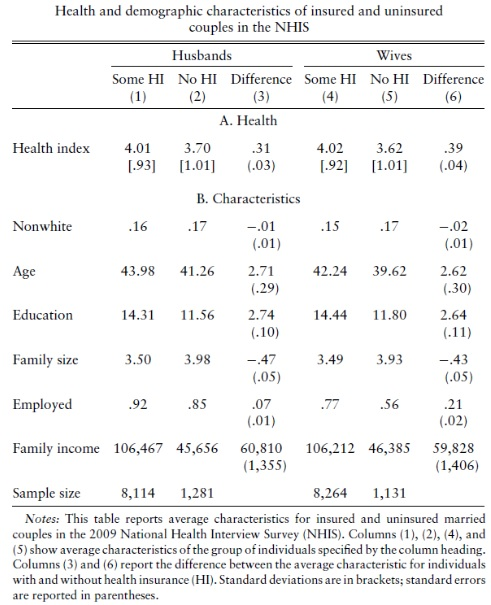
\includegraphics[width=10cm,height=6.5cm,keepaspectratio]{RAND Table 1} 

\column{.45\textwidth}
\begin{itemize}
	\item Americans with insurance seem to be healthier 
	\item But there are differences in people with and without coverage!
	\item those with insurance have higher education, higher income, ...
\end{itemize}

\end{columns}

\end{frame}

%------------------------------------------------
\begin{frame}
\frametitle{How to measure causal effect}
First, we have to establish how to write down our variables:
\begin{itemize}
\item Outcome: \textit{Y} (in our example: health)
\item {$Y_i$}: health of individual \textit{i}
\item every person \textit{i} has two potential outcomes: $Y_0_i$ (without insurance) and $Y_1_i$ (with insurance)
\item the causal effect of insurance: $Y_1_i$ - $Y_0_i$
\end{itemize}
\end{frame}
%------------------------------------------------
\begin{frame}
\frametitle{Example}
Imagine two people: Max and Moritz. Max is very healthy and fit, Moritz has always had a fragile health.
They can both decide whether to acquire health insurance or not. Let's have a look at their health index (ranked from poor (1) to excellent (5):
\begin{itemize}
\item $Y_{0,~\mathrm{Max}}$ = 5 and $Y_{1,~\mathrm{Max}}$ = 5
\item $Y_{0,~\mathrm{Moritz}}$ = 3 and $Y_{1,~\mathrm{Moritz}}$ = 4 
\item the effect of getting insurance for Max = 0 and for Moritz = 1
\item problem: \textit{selection bias} between those two
\item Moritz has worse health even if both of them decide not to get insurance
\end{itemize}

\end{frame}
%------------------------------------------------
\begin{frame}
\frametitle{Average Causal Effects}
The problem of the selection bias is consistent also in groups. Therefore we look at the \textbf{average causal effects}. In a group of \textit{n} people, the average causal effect is:

$$Avg_n[Y_1_,_i - Y_0_,_i] = \frac{1}{n} \sum_{i=1}^n [Y_1_,_i - Y_0_,_i]~~~~~~~~~~~~~~~~~~~~~~~~~~~~~~~~~~$$
$$=\frac{1}{n}\sum_{i=1}^{n}{[Y_1_,_i]} - \frac{1}{n} \sum_{i=1}^n [Y_0_,_i]~~~~~~~~~~~~~~~~~~~~~~~~~~~~~~~~~~$$
\begin{itemize}
	\item We compare average health in a scenario where everybody in the group does and does not have health insurance
	\item to make this comparison easier, we will use a \textit{dummy variable}, $D_i$
	\item $D_i=1$ means insured, $D_i=0$ means uninsured
\end{itemize}
\end{frame}



%------------------------------------------------
\begin{frame}
\frametitle{Difference in group means}
We can now use Dummies for the average in the two groups ($Avg_n[Y_i|D_i=1]$ for the insured and $Avg_n[Y_i|D_i=0]$ for the uninsured).\\~\\

Therefore the difference in group means would be:
$$Avg_n[Y_i|D_i=1]-Avg_n[Y_i|D_i=0]$$
$$=Avg_n[Y_{1i}|D_i=1]-Avg_n[Y_{0i}|D_i=0]$$

\end{frame}
%------------------------------------------------

\begin{frame}
\frametitle{constant-effects assumption}
We are interested in $Avg_n[Y_{1i}-Y_{0i}]$, therefore we can imagine that people with insurance are healthier than people without an insurance.

Let's say that everyone is healthier through the insurance by the amount \kappa.

We can use the \textit{constant-effects assumption}

$$Y_{1i} = Y_{0i} + \kappa$$

$\kappa$ stands for the individual and average causal effect of insurance on health.

\end{frame}
%------------------------------------------------
\begin{frame}
\frametitle{Oranges \& Apples}

Using the constant-effects models we can substitute $Avg_n$ and get:
$$Avg_n[Y_{1i}|D_i=1]-Avg_n[Y_{0i}|D_i=0]$$
$$= {\kappa +Avg_n[Y_{0i}|D_i=1]} - Avg_n[Y_{0i}|D_i=0]$$

\begin{itemize}

	\item But: difference in group means = average causal effect + selection bias!

	\item $Y_{0i}$ is any characterictic related to health that's not insurance and therefore comparing outcomes for two groups with different $Y_{0i}$ is comparing oranges with apples.

	\item Even if the insurance effect $\kappa$ was zero, our groups would differ in their health.
\end{itemize}

\end{frame}
%------------------------------------------------
\begin{frame}
\frametitle{Randomized Experiments}
\begin{itemize}
\item Experimental random assignment eliminates the selection bias.

\item Idea: we start with a sample of people that is currently uninsured
\item we would give health insurance to a randomly chosen subset of this sample
\item due to random assignment we can compare these groups ceteris paribus (they differ only in their health insurance status)
\item Watch out: two make two randomly chosen groups comparable, they have to be large enough (Law of Large Numbers LLN)!
\end{itemize}

\end{frame}

%------------------------------------------------
\begin{frame}
\frametitle{Law of Large Numbers}
\begin{itemize}
\item The LLN shows the behavior of sample averages in relation to sample size
\item For example, imagine to play dice: everytime you throw the dice, you write down your result and average these results
\item You have six possible outcomes (numbers 1 to 6) but after enough throws you would expect to get 3,5 on average!
\item this average value represents the mathematical expectation
\end{itemize}


\end{frame}

%------------------------------------------------
\begin{frame}
\frametitle{mathematical and conditional expectations}
\begin{block}{mathematical expectation}
The mathematical expectation of a variable $E[Y_i]$ is the average obtained if everyone in the survey population from which the sample os drawn was to be enumerated.
\end{block}

\begin{block}{conditional expectation}
The conditional expectation of a variable $Y_i$, given a dummy variable $D_i=1$, is written $E[Y_i|D_i=1]$. This expression stands for the average of $Y_i$ in the population that has $D_i =1$. 
\end{block}

\begin{block}{random assignment}
As randomly assigned treatment and control group come from the same population, they are the same in every way, also in their expected $Y_{0i}$. Therefore, their conditional expectations $E[Y_{0i}|D_i=1]$ and $E[Y_{0i}|D_i=0]$ are the same.
\end{block}


\end{frame}

%------------------------------------------------
\begin{frame}
\frametitle{random assignment eliminates selection bias}
When $D_i$ is randomly assigned, $E[Y_{0i}|D_i=1] = E[Y_{0i}|D_i=0]$ and therefore the difference in expectations by the treatment shows the causal effect of the treatment.\\~\\

$E[Y_i|D_i=1]-E[Y_i|D_i=0]$

$=E[Y_{1i}|D_i=1] - E[Y_{0i}|D_i=0]$

$=E[Y_{0i} + \kappa|D_i=1] - E[Y_{0i}|D_i=0]$

$=\kappa$ 

\begin{itemize}
\item Conclusion: when the sample is large enough, due to the LLN, the selection bias disappears in a randomized experiment! Random assignment ensures that the mix of the individuals in the different groups is the same.
\item when analyzing data from a randomized trial, you should always be checking for balance to make sure your treatment and control groups look similar.
\end{itemize}
\end{frame}



%------------------------------------------------
\begin{frame}
\frametitle{The RAND Health Insurance Experiment}
\begin{itemize}
\item We will now talk about the RAND Health Insurance Experiment  in which 3958 participants were randomly assigned to health different health insurance plans.
\item The experiment was carried out from 1974 to 1982 in the USA.
\item Participants were randomly assigned into 14 insuranceplans. 
\item These can be roughly categorized into 4 types:
	\begin{itemize} 
	\item Catastrophic: families pay 95 \% of their healthcare costs themselves (capped at \$1000)
	\item uninsured: families pay 95 \% of their healthcare costs themselves (capped at \$450)
	\item Coinsurance: families pay 25-50 \% if their healthcare costs themselves (capped at \$1000)
	\item Free: would be similar to the German health insurance
	\end{itemize}
\end{itemize}

\end{frame}
%------------------------------------------------
\begin{frame}
\frametitle{The RAND experiment: first glance}
\begin{columns}
\column{.5\textwidth}
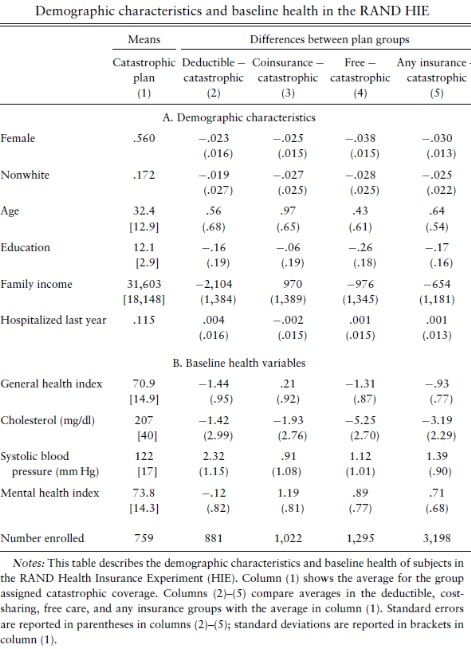
\includegraphics[width=10cm,height=6.5cm,keepaspectratio]{RAND Table 2} 

\column{.45\textwidth}
\begin{itemize}
	\item first step: checking for balance
	\item the participants in the different plans seem to be similar (Panel A)
	\item values in the brackets are \textit{standard errors} so that you can check whether a difference is large enough to be \textit{statistically significant}
	\item differences larger than two standard errors are \textit{statistically significant}
\end{itemize}

\end{columns}
\end{frame}
%------------------------------------------------
\begin{frame}
\frametitle{The RAND experiment: first glance}
\begin{columns}
\column{.5\textwidth}
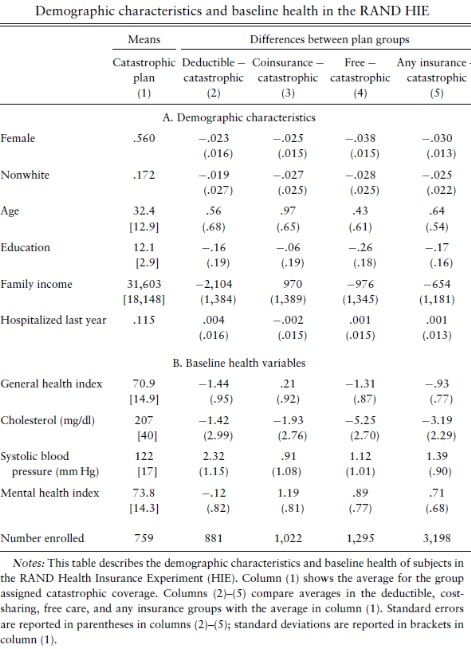
\includegraphics[width=10cm,height=6.5cm,keepaspectratio]{RAND Table 2} 

\column{.45\textwidth}
\begin{itemize}
	\item first step: checking for balance
	\item good balance in pre-treatment index of general health (Panel B)
	\item no statistically significant differences in pre-treatment cholesterol, etc. 
\end{itemize}

\end{columns}
\end{frame}
%------------------------------------------------
\begin{frame}
\frametitle{The RAND experiment}
\begin{columns}
\column{.5\textwidth}
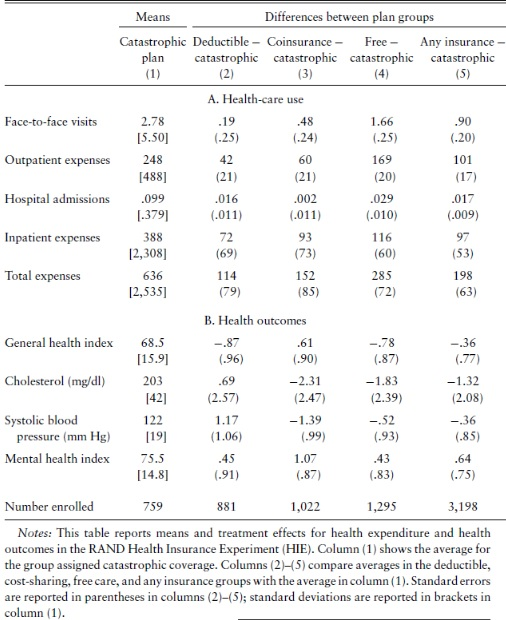
\includegraphics[width=10cm,height=6.5cm,keepaspectratio]{RAND Table 3} 

\column{.45\textwidth}
\begin{itemize}
	\item Now we observe the health expenditure \& outcomes
	\item with more generous insurance plan, more health care use (Panel A)
	\item the health care use was different among insurance groups
	\item but we can't find a great difference between groups in the health outcomes
\end{itemize}

\end{columns}
\end{frame}
%------------------------------------------------
\begin{frame}
\frametitle{Does health insurance make people healthier?}
\begin{itemize}
	\item after looking at the results of the RAND Health Insurance Experiment, generous health care might have some unintended and undesirable consequences. 
	\item due to increased health care use the costs would go up without improving health care outcomes.
	\item before trying to give a final answer to whether health insurance makes people healthier we will have a look at another experiment.
\end{itemize}

\end{frame}

%------------------------------------------------

%zweite section OHG
\section{The Oregon Trail}
\begin{frame}
\frametitle{The Oregon Trail}
\newline 
\begin{itemize}
	\item RAND might have missed the mark
  \item Today´s uninsured Americans differ considerably from the RAND population: most of the
uninsured are younger, less educated, poorer, and less likely to be
working. 
  \item The value of extra health care in such a group might be very
different than for the middle class families that participated in the RAND Study
  \item What´s the effect of insuring the currently uninsured?
  \item Solution: Oregon Health Plan (OHP) lottery
\end{itemize}

\end{frame}

%---------------------------------------------------

\begin{frame}
\frametitle{Oregon Health Plan}
\begin{itemize}
	\item State of Oregon offered Medicaid of thousands of randomly chosen people in a lottery
	\item Only Oregon residents 19-64 years old could apply
	\item Winners could apply for Medicaid $\rightarrow$ coverage
was not automatic, even for lottery winners
	\item Out of 75000 Applicants 30000 were randomly selected and invited to apply. The other 45000 constitute the control group.
	\item Are OHP lottery winners more likely to end up insured as a result of winning?
\end{itemize}


\end{frame}

%---------------------------------------------------
\begin{frame}

\begin{columns}
\column{.5\textwidth}
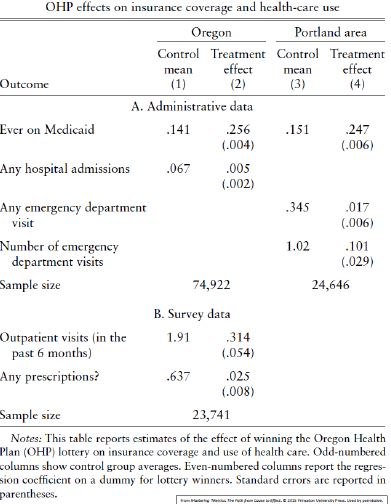
\includegraphics[width=10cm,height=6.5cm,keepaspectratio]{OHP Table 1} 

\column{.45\textwidth}
\begin{itemize}
	\item OHP winners rather insured than lottery losers
	\item Treatment group used more healthcare services
	\item More emergency dep. visits
\end{itemize}

\end{columns}

\end{frame}

%---------------------------------------------------

\begin{frame}
\frametitle{But did that make them healthier?}
\begin{columns}
\column{.5\textwidth}
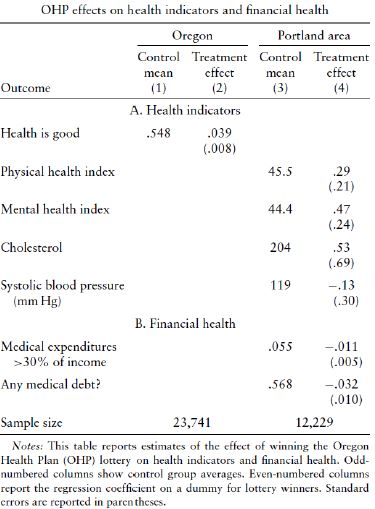
\includegraphics[width=10cm,height=6.5cm,keepaspectratio]{OHP Table 2}

\column{.45\textwidth}
\begin{itemize}
	\item not really
	\item statistically insignificant changes for physical and mental health
	\item changes in financial health could account for improved mental
health
\end{itemize}

\end{columns}

\end{frame}

%---------------------------------------------------

\begin{frame}
\frametitle{Results}
\begin{itemize}
	\item Both experiments produces similar results
	\item Use of healthcare services increases sharply in response to insurance coverage
	\item But neither experiment reveals much of an insurance effect on physical health.
	\item These studies suggest that subsidized public health insurance should not be expected
to yield a dramatic health dividend.
\end{itemize}

\end{frame}

%---------------------------------------------------

\begin{frame}
\frametitle{In a nutshell}
\begin{itemize}
	\item \textbf{Causal inference} compares potential outcomes, descriptions of the world when alternative roads are taken.
	\item We cannot compare those who took one road with those who took another
	\item These comparisons are often contaminated by \textbf{selection
bias}, that is, differences between treated and control subjects that
exist even in the absence of a treatment effect.
	\item \textbf{Random assignment} to treatment and control
conditions eliminates selection bias.
	\item But we should still \textbf{check for balances}.
\end{itemize}


\end{frame}

%Appendix
%---------------------------------------------------

\section{Appendix}
\begin{frame}
\frametitle{Mastering Interference}
\begin{itemize}
	\item How can we decide whether statistical results constitute strong evidence or are a lucky draw, unlikely to be replicated in repeated samples? 
	\item How much sampling variance should we expect?
	\item Goal: The quantification of the uncertainty associated
with a particular sample average and groups of averages and
the differences among them.
	\item For example the RAND: Instead of studying the
many millions of families, just about 2000 Families were selected at random and
then randomly allocated to one of 14 plans or treatment groups.
	\item Two sorts of randomness: Random sampling and random
assignment.
\end{itemize}

\end{frame}

\begin{frame}
\frametitle{Random Sampling}
\begin{itemize}
	\item Population mean of a variable is called mathematical expectation
	\item The Expectation of a variable $Y_i$ we write $E[Y_i]$.
	\item Unbiasedness of the Sample Mean $E[\bar{Y}] = E[Y_i]$
\end{itemize}

\end{frame}


%Mathe Latex vom 16 April Max
%------------------------------------------------

\begin{frame}
\frametitle{Random Sampling}
\begin{itemize}
	\item Population mean of a variable is called mathematical expectation
	\item The Expectation of a variable $Y_i$ we write $E[Y_i]$.
		\begin{itemize}
			\item[\textbullet] $E[Y_i]$ \triangleright Whole Population\triangleright Parameter,\ fixed\ feature\\
		\end{itemize}
		\begin{itemize}
			\item[\textbullet] $E[\bar{Y}]$ \triangleright Sample\ n \triangleright Sample\ Statistic \\
		\end{itemize}
	\item The sample average, $E[\bar{Y}]$, is a good estimator of $E[Y_i]$ (in statistics, an estimator is any
function of sample data used to estimate parameters).
	
\end{itemize}

\end{frame}

%--------------------------------------------

\begin{frame}
\frametitle{Random Sampling}

\begin{itemize}
	\item LLN tells us that in large samples, the sample average is likely to be very close to the corresponding population mean.
	\item  A related property is that the expectation of $E[\bar{Y}]$ is also $E[Y_i]$
	\item if we were to draw infinitely many random samples, the average of the resulting $E[\bar{Y}]$ across
draws would be the underlying population mean.
	\item When a sample statistic has expectation equal to the corresponding population parameter, its said to be an unbiased estimator of that parameter.
	\item Unbiasedness of the Sample Mean $E[\bar{Y}] = E[Y_i]$
\end{itemize}

\end{frame}

%--------------------------------------------

\begin{frame}
\frametitle{Random Sampling}
\begin{itemize}
	\item Unbiasedness tells us that these deviations are not systematically up or down; rather, in repeated samples they average out to zero
	\item This is different from the LLN (Law of large Numbers)
	\item LLN says that the sample mean gets closer and closer to the population mean as the sample size grows.
\end{itemize}

\end{frame}

%--------------------------------------------

\begin{frame}
\frametitle{Measuring Variability}
\begin{itemize}
	\item To measure variability we need to look at average squared deviations from the
mean, in which positive and negative gaps get equal weight. 
	\item The resulting summary of variability is called variance.
	\item Sampling variance of sample average depends on the variance of the underlying observations $\sigma^2_y$ and the sample size $n$.
\end{itemize}


\end{frame}

%--------------------------------------------

\begin{frame}
\frametitle{Measuring Variability}
The sample variance of $Y_i$ in a sample size of n is defined as: \\
\vspace{0.5cm} 
%\begin{equation*}
\hspace{3cm}${V(Y_i)^2=\frac{1}{n}\[\sum^{n}_{i=1}\](Y_i-\bar{Y})^2}$ \\~\\
%\end{equation*} \\~\\
\vspace{0.5cm} 
Because the expectation of the sample mean $E(\bar{Y})$ is $E[Y_i]$ the population variance of the sample mean can be written as: \\
%\begin{equation*}
$$V(\bar{Y})=E[(\bar{Y}-E[\bar{Y}])^2]=E[(\bar{Y}-E[Y_i])^2]$$ \\~\\
%\end{equation*} \\

\begin{itemize}
	\item $V(Y_i)or(\sigma^2_y)$ denotes the variance of the underlying data, while $V(\bar{Y})$ is written for the variance of the sample mean
\end{itemize}


\end{frame}

%--------------------------------------------
\begin{frame}
\frametitle{Measuring Variability}
\begin{itemize}
	\item Simplified, the standard error of the sample mean can be written as: 
		%\begin{equation*}
		$$SE(\bar{Y})=\frac{\sigma_y}{\sqrt{n}}$$
		%\end{equation*} \\
		
	\item This summarizes the variability in an estimate due to random sampling
	\item Every estimate has an associated standard error
	\item But: Usually most quantities are unknown and must be estimated 
	\item Therefore: We work with an estimated standard error:
		%\begin{equation*}
		$$\hat{SE}(\bar{Y})=\frac{S(Y_i)}{\sqrt{n}}$$
		%\end{equation*} \\
\end{itemize}
\end{frame}


% ab hier neu eingefugt am 20.04.
%------------------------------------------------
\begin{frame}
\frametitle{t-Statistic}

\begin{itemize}
	\item Now that we know how to measure variability, we just need to interpret it.
	\item Here: $E[Y_i]=\mu$
	\item This constitutes a working hypothesis and is a reference point called the null hypothesis
	\item Any t-Statistic for the sample mean under the working hypothesis is constructed as:\\
		%\begin{equation*}
		$$t(\mu)=\frac{\bar{Y}-\mu}{SE(\bar{Y})}$$
		%\end{equation*} \\
	\item The t-statistic is the ratio of the sample mean to its estimated standard error.
	\item With the t-statistic, we can interpret the results.
\end{itemize}

\end{frame}

%--------------------------------------------

\begin{frame}
\frametitle{Central Limit Theorem}
\begin{itemize}
	\item If $E[Y_i]=\mu$ and the sample size is large:
	\item The quantity ${t(\mu)}$ has a sampling distribution that is very close to a bell-shaped standard normal distribution. \\
	\item This is called the Central Limit Theorem (CLT)
	\item This allows us to make an empirically informed decision as to whether the available
data support or cast doubt on the hypothesis that $E[Y_i]$ equals $\mu$.
\end{itemize}

\end{frame}

%--------------------------------------------

\begin{frame}
\frametitle{When is it significant?}

\begin{itemize}
	\item The standard normal distribution has a mean of 0 and standard
deviation of 1. 
	\item With any standard normal variable, values larger than ±2 are highly unlikely.
	\item Realizations larger than 2 in absolute value appear only about $5\%$ of the time. 
  \item Because the t-statistic is close to normally distributed, we similarly expect it to fall between about ±2
most of the time. 
	\item Therefore, any t-statistic larger than about 2 (in absolute value) is too unlikely to be consistent with the null hypothesis used to construct it. 
	\item When the null hypothesis is μ = 0 and the t-statistic exceeds 2 in absolute value, we say the sample mean is \textbf{significantly different from zero (statistically significant)}.
\end{itemize}

\end{frame}

%--------------------------------------------

\begin{frame}
\frametitle{Confidence intervalls}

\begin{itemize}
	\item The other side of this looks as follows
	\item Instead of checking whether the sample is consistent with a specific
value of $\mu$, we can construct the set of all values of $\mu$ that are consistent
with the data.
	\item That is called a confidence interval for $E[Y_i]$:
		\begin{equation*}
		[\bar{Y}-2\times{\hat{SE}(\bar{Y})},\bar{Y}+2\times{\hat{SE}(\bar{Y})}]
		\end{equation*} \\
	\item When calculated in repeated samples, the interval should contain $E[Y_i]$ about 95\% of the time.
	\item This interval is therefore said to be a 95\% confidence interval for the population mean.
\end{itemize}

\end{frame}

%--------------------------------------------

\begin{frame}
\frametitle{Pairing Off}

\begin{itemize}
	\item Another option to measure if treatment changes outcomes:
	\item Hereby we use the treatment and the control group: 
	\item $\bar{Y}^1$ is the treatment group mean, $\bar{Y}^0$ is the control group mean, with the sample size being $n=n^1 + n^0$
	\item The difference between $\bar{Y}^1$ and $\bar{Y}^0$ is an estimate of the causal effect of the treatment.
	\item If the treatment changes outcomes, there also must be different values for $\mu^1$ and $\mu^0$. 
	%\item So we check the hypothesis that $\mu^1$ = $\mu^0$ by looking for statistically significant differences in the corresponding sample average.
\end{itemize}

\end{frame}

%--------------------------------------------

\begin{frame}
\frametitle{Pairing Off}

\begin{itemize}
	\item Under the null hypothesis that $\mu^1 $-$ \mu^0$ is equal to the value $\mu$, the t-statistic for a difference in means is: \\
		\begin{equation*}
			t(\mu)=\frac{\bar{Y}^1-\bar{Y}^0-\mu}{{\hat{SE}(\bar{Y}^1-\bar{Y}^0)}}
		\end{equation*} \\
	\item With the $\hat{SE}$ being the estimated standard error: \\
		\begin{equation*}
			\hat{SE}(\bar{Y}^1-\bar{Y}^0) = S(Y_i)\sqrt{\frac{1}{n_1}+\frac{1}{n_0}}
		\end{equation*} \\
	\item $S(Y_i)$ in this case means the pooled sample standard deviation = both treatment and control group combined.
	\item We use this t-statistic to test working hypotheses about $\mu_1$ $-$ $\mu_0$ and to
construct confidence intervals for this difference.
\end{itemize}

\end{frame}
%--------------------------------------------

\begin{frame}
\frametitle{Pairing Off}
\begin{itemize}
	\item When the null hypothesis is one of equal means $(\mu = 0)$, the statistic $t(\mu)$ equals the
difference in sample means divided by the estimated standard error of this difference. \\
	\item When the t-statistic is large enough to reject a difference of zero, we say the estimated difference is statistically significant. \\
	\item Lack of statistical significance reflects lack of statistical precision (high
sampling variance).
\end{itemize}

\end{frame}
%----------------------------------------------------------------------------------------

\begin{frame}
\Huge{\centerline{Thank you very much for listening}}
\end{frame}

%----------------------------------------------------------------------------------------

\end{document} 